\message{ !name(NeuriImag-1111-SBM.tex)}\documentclass{beamer}

% Beamer style
%\usetheme[secheader]{Madrid}
\usetheme{CambridgeUS}
\usecolortheme[rgb={0.65,0.15,0.25}]{structure}
%\usefonttheme[onlymath]{serif}
\beamertemplatenavigationsymbolsempty
%\AtBeginSubsection

% Packages
%\usepackage[french]{babel}
\usepackage[latin1]{inputenc}
\usepackage{color}
\usepackage{dsfont, stmaryrd}
\usepackage{amsmath, amsfonts, amssymb}
\usepackage{stmaryrd}
\usepackage{epsfig}
\usepackage{url}
\usepackage{/Latex/astats}
%\usepackage[all]{xy}
\usepackage{graphicx}

% Commands
\definecolor{darkred}{rgb}{0.65,0.15,0.25}
%\newcommand{\emphase}[1]{\textcolor{darkred}{#1}}
\newcommand{\emphase}[1]{{#1}}
\newcommand{\paragraph}[1]{\textcolor{darkred}{#1}}
\newcommand{\refer}[1]{\textcolor{blue}{\sl \cite{#1}}}
\newcommand{\Refer}[1]{\textcolor{blue}{\sl #1}}
\newcommand{\newblock}{}

% Symbols
\newcommand{\Abf}{{\bf A}}
\newcommand{\Beta}{\text{B}}
\newcommand{\Bcal}{\mathcal{B}}
\newcommand{\BIC}{\text{BIC}}
\newcommand{\dd}{\text{d}}
\newcommand{\dbf}{{\bf d}}
\newcommand{\Dcal}{\mathcal{D}}
\newcommand{\Esp}{\mathbb{E}}
\newcommand{\Ebf}{{\bf E}}
\newcommand{\Ecal}{\mathcal{E}}
\newcommand{\Gcal}{\mathcal{G}}
\newcommand{\Gam}{\mathcal{G}\mbox{am}}
\newcommand{\Ibb}{\mathbb{I}}
\newcommand{\Ibf}{{\bf I}}
\newcommand{\ICL}{\text{ICL}}
\newcommand{\Cov}{\mathbb{C}\text{ov}}
\newcommand{\Corr}{\mathbb{C}\text{orr}}
\newcommand{\Var}{\mathbb{V}}
\newcommand{\Vsf}{\mathsf{V}}
\newcommand{\pen}{\text{pen}}
\newcommand{\Fcal}{\mathcal{F}}
\newcommand{\Hbf}{{\bf H}}
\newcommand{\Hcal}{\mathcal{H}}
\newcommand{\Jcal}{\mathcal{J}}
\newcommand{\Kbf}{{\bf K}}
\newcommand{\Lcal}{\mathcal{L}}
\newcommand{\Mcal}{\mathcal{M}}
\newcommand{\mbf}{{\bf m}}
\newcommand{\mum}{\mu(\mbf)}
\newcommand{\Ncal}{\mathcal{N}}
\newcommand{\Nbf}{{\bf N}}
\newcommand{\Nm}{N(\mbf)}
\newcommand{\Ocal}{\mathcal{O}}
\newcommand{\Obf}{{\bf 0}}
\newcommand{\Omegas}{\underset{s}{\Omega}}
\newcommand{\Pbf}{{\bf P}}
\newcommand{\Pcal}{\mathcal{P}}
\newcommand{\Qcal}{\mathcal{Q}}
\newcommand{\Rbb}{\mathbb{R}}
\newcommand{\Rcal}{\mathcal{R}}
\newcommand{\sbf}{{\bf s}}
\newcommand{\Sbf}{{\bf S}}
\newcommand{\Scal}{\mathcal{S}}
\newcommand{\Ucal}{\mathcal{U}}
\newcommand{\Vcal}{\mathcal{V}}
\newcommand{\Tbf}{{\bf T}}
\newcommand{\ubf}{{\bf u}}
\newcommand{\Ubf}{{\bf U}}
\newcommand{\Wbf}{{\bf W}}
\newcommand{\xbf}{{\bf x}}
\newcommand{\Xbf}{{\bf X}}
\newcommand{\ybf}{{\bf y}}
\newcommand{\Ybf}{{\bf Y}}
\newcommand{\zbf}{{\bf z}}
\newcommand{\Zbf}{{\bf Z}}
\newcommand{\betabf}{\mbox{\mathversion{bold}{$\beta$}}}
\newcommand{\pibf}{\mbox{\mathversion{bold}{$\pi$}}}
\newcommand{\Sigmabf}{\mbox{\mathversion{bold}{$\Sigma$}}}
\newcommand{\gammabf}{\mbox{\mathversion{bold}{$\gamma$}}}
\newcommand{\mubf}{\mbox{\mathversion{bold}{$\mu$}}}
\newcommand{\nubf}{\mbox{\mathversion{bold}{$\nu$}}}
\newcommand{\Thetabf}{\mbox{\mathversion{bold}{$\Theta$}}}
\newcommand{\thetabf}{\mbox{\mathversion{bold}{$\theta$}}}
\newcommand{\BP}{\text{BP}}
\newcommand{\EM}{\text{EM}}
\newcommand{\VEM}{\text{VEM}}
\newcommand{\VBEM}{\text{VB}}
\newcommand{\cst}{\text{cst}}
\newcommand{\obs}{\text{obs}}
\newcommand{\ra}{\emphase{\mathversion{bold}{$\rightarrow$}~}}
\newcommand{\QZ}{Q_{\Zbf}}
\newcommand{\Qt}{Q_{\thetabf}}

% Directory
\newcommand{\fignet}{/RECHERCHE/RESEAUX/Exposes/Figures}
\newcommand{\figmotif}{/RECHERCHE/RESEAUX/Motifs/FIGURES}


%--------------------------------------------------------------------
\title[Variational inference for SBM]{Variational
  inference for the Stochastic Block-Model}  

\author{S. Robin}

\institute[AgroParisTech / INRA]{AgroParisTech / INRA \\
  \bigskip
  \begin{tabular}{ccccc}
    
\epsfig{file=/RECHERCHE/RESEAUX/Exposes/Figures/LogoINRA-Couleur.ps,
      width=2.5cm} & 
    \hspace{.5cm} &
    
\epsfig{file=/RECHERCHE/RESEAUX/Exposes/Figures/logagroptechsolo.eps,
      width=3.75cm} & 
    \hspace{.5cm} &
    \epsfig{file=/RECHERCHE/RESEAUX/Exposes/Figures/Logo-SSB.eps,
      width=2.5cm} \\ 
  \end{tabular} \\
  \bigskip
  }

\date[SemStat'11, Paris]{Neuroimaging - Genetics Workshop, Paris, November 2011}
%--------------------------------------------------------------------

%--------------------------------------------------------------------
%--------------------------------------------------------------------
\begin{document}

\message{ !name(NeuriImag-1111-SBM.tex) !offset(-3) }

%--------------------------------------------------------------------
%--------------------------------------------------------------------

%--------------------------------------------------------------------
\frame{\titlepage}

% %--------------------------------------------------------------------
% \frame{ \frametitle{Outline}
%   \tableofcontents}

%--------------------------------------------------------------------
\section{Stochastic block model}
\frame{\frametitle{Stochastic block model (SBM)}}
%--------------------------------------------------------------------
\subsection{Understanding network structure}
%--------------------------------------------------------------------
\frame{\frametitle{Understanding network structure}

  \begin{itemize}
  \item Network constitute a natural way to depict interactions
    between entities.
  \item They are now present in many scientific fields (biology,
    sociology, communication, economics, ...).
  \item Most observed networks display an heterogeneous topology, that
    one would like to decipher and better understand. \pause
  \end{itemize}
  \begin{tabular}{ll}
    %\hspace{-.5cm}
    \begin{tabular}{p{.5\textwidth}}
      \paragraph{Dolphine social network.} \\
      %\epsfig{file=../Figures/NeG04-Fig11.ps, clip=, width=.5\textwidth}
      \epsfig{file=../Figures/NeG04-PhysRevE-Fig11.ps, clip=,
        width=.4\textwidth, bbllx=60, bblly=590, bburx=295,bbury=745}\\
      \refer{NeG04}
    \end{tabular}
    & 
    \hspace{-.5cm}
    \begin{tabular}{p{.5\textwidth}}
      \paragraph{Hyperlink network.} \\
      %\epsfig{file=../Figures/NeG04-Fig13.ps, clip=, width=.5\textwidth}
      \epsfig{file=../Figures/NeG04-PhysRevE-Fig13.ps, clip=,
        width=.4\textwidth, bbllx=50, bblly=545, bburx=300,bbury=745} 
    \end{tabular} 
  \end{tabular} 
  }

%--------------------------------------------------------------------
\frame{\frametitle{Modelling network heterogeneity}
  \paragraph{Latent variable models} allow to capture
  the underlying structure of a network.

  \bigskip\pause
  \paragraph{General setting} for binary graphs (\refer{BJR07}): \pause
  \begin{itemize}
  \item an \emphase{latent (unobserved) variable $Z_i$} is associated
    with each node:
    $$
    \{Z_i\} \text{ i.i.d. } \sim \pi 
    $$
  \item the edges \emphase{$X_{ij}$ are independent conditionally} to the
    $Z_i$'s:
    $$
    \{X_{ij}\} \text{ independent } | \{Z_i\}: X_{ij}  \sim 
    \Bcal[\gamma(Z_i, Z_j)]
    $$
  \end{itemize}

  \bigskip\pause
  \paragraph{Continuous (\refer{HRH02}):} ($\simeq$ PCA)
  $$
  Z_i \in \Rbb^d, \qquad \text{logit}[\gamma(z, z')] = a - |z-z'|
  $$

  \bigskip\pause
  \paragraph{Discrete (\refer{NoS01}):} (\ra finite mixture $=$
  \emphase{SBM})
  $$
  Z_i \in \{1, \dots, K\}, \qquad \gamma(k, \ell) = \gamma_{k\ell}.
  $$
  }

%--------------------------------------------------------------------
\frame{\frametitle{(Valued) Stochastic Block-Model (SBM)}
  \paragraph{Discrete-valued latent labels:}
  each node $i$ belong to class $k$ with probability $\pi_k$:
  $$
  \{Z_i\}_i \mbox{ i.i.d.}, \qquad Z_i \sim \Mcal(1; \pibf)
  $$
  where $\pibf = (\pi_1, \dots \pi_K)$.

  \bigskip\pause
  \paragraph{Observed edges:} $\{X_{ij}\}_{i,
    j}$ are conditionally independent given the $Z_i$'s:
  $$
  (X_{ij} \;|\; Z_i = k, Z_j = \ell) \sim f_{k\ell}(\cdot)
  $$
  where $f_{k\ell}(\cdot)$ is some parametric distribution
  $f_{k\ell}(x) = f(x; \gamma_{k\ell})$, e.g.
  $$
  (X_{ij} \;|\; Z_i = k, Z_j = \ell) \sim \Bcal(\gamma_{k\ell})
  \qquad (\text{binary graph})
  $$
  We denote   $\gammabf = \{\gamma_{k\ell}\}_{k, \ell}.$
  
  \bigskip\pause
  \paragraph{Inference:} We want to estimate
  $$
  \thetabf = (\pibf, \gammabf)
  \qquad \text{and} \qquad
  P(\Zbf | \Xbf).
  $$
  }

%-------------------------------------------------------------------- 
\frame{ \frametitle{SBM for a binary social network}

  \vspace{-.5cm}
  \begin{tabular}{ll}
%      \paragraph{An example.}
%      & 
%      \\
      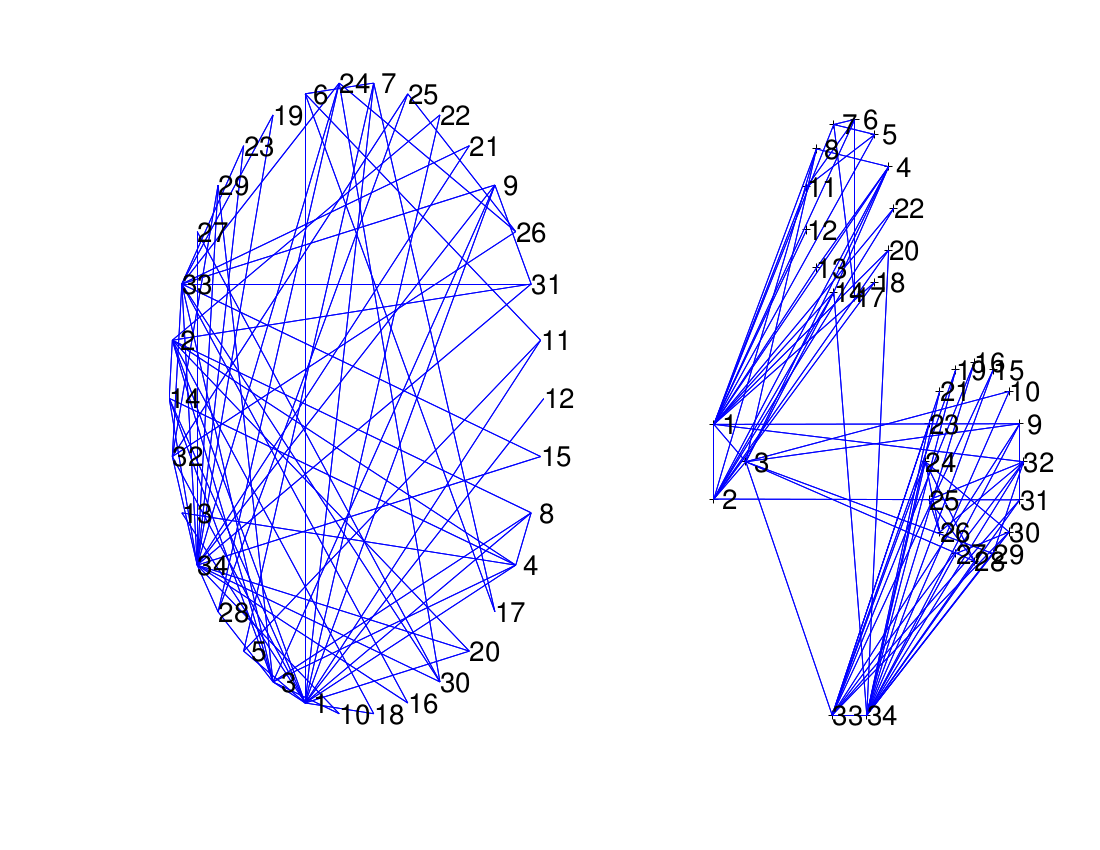
\epsfig{file = \fignet/Karate-Graph.eps, clip=, width=3.5cm,
        height=5cm, angle=270, bllx=50, bblly=80, bburx=530,
        bbury=420} 
      &
      \onslide+<2->{
        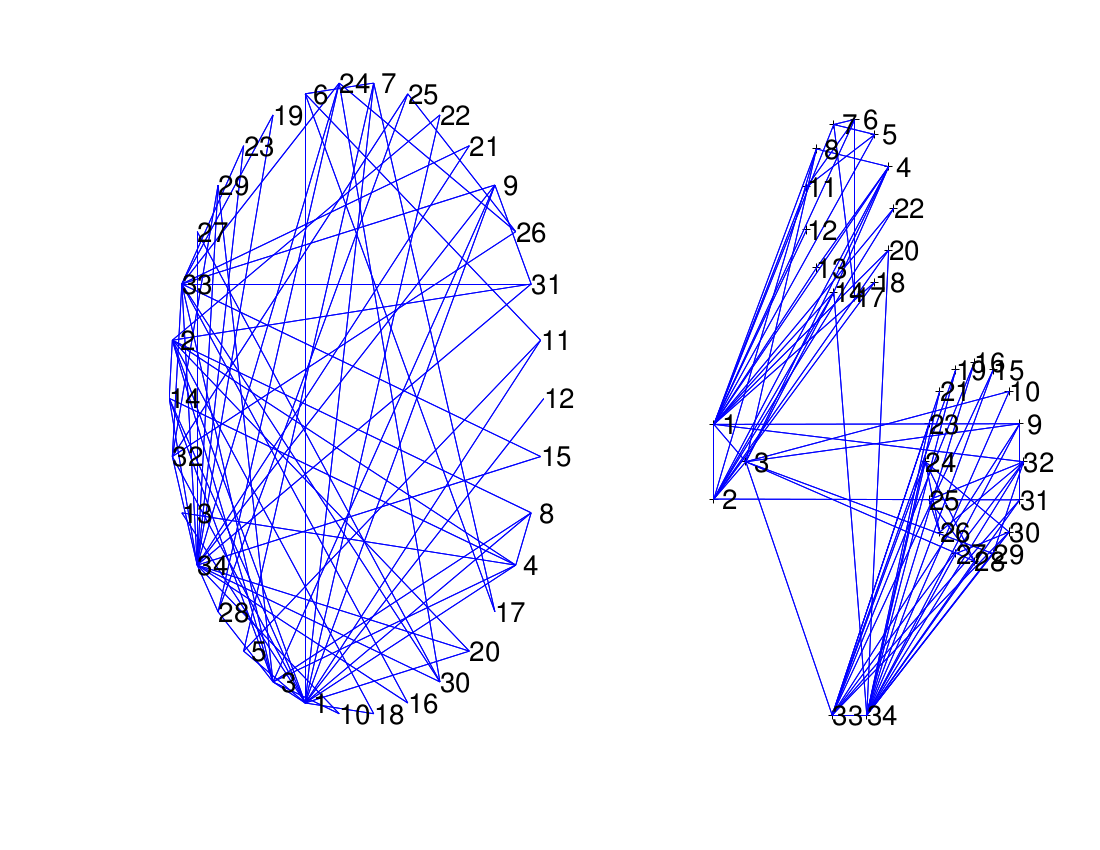
\epsfig{file = \fignet/Karate-Graph.eps, clip=, width=3.5cm,
          height=5cm, angle=270, bllx=70, bblly=490, bburx=530,
          bbury=770} 
        }
      \\     
      ~\\
      \begin{tabular}{p{.4\textwidth}}
        \paragraph{Zachary data.} Social binary network of friendship
        within a sport club. \\ 
        \\ 
        \onslide+<2->{
          \paragraph{Results.} 
          The split is recovered and the role of few leaders is
          underlined. 
          }
      \end{tabular}
      & 
      \begin{tabular}{p{.5\textwidth}}
        \onslide+<3->{
          {\small
            \begin{tabular}{c|rrrr}
              (\%) & \multicolumn{4}{c}{$\widehat{\gamma}_{k\ell}$} \\
              $k / \ell$ &  {1} & 2 & 3 &  4 \\
              \hline
              {1} &  {100} &   {53} &  {16} & {16} \\  
              {2} & - &  {12} & {0} & {7}  \\  
              3 & - & - & 8 & 73 \\
              4 & - & - & - & 100\\
              \hline
              $\widehat{\pi}_{\ell}$        & 9 &  38       & 47    & 6     \\
            \end{tabular}
            }
          }
    \end{tabular}
  \end{tabular}

%   \vspace{-1cm}\hspace{-1cm}
%   \begin{tabular}{c}
%     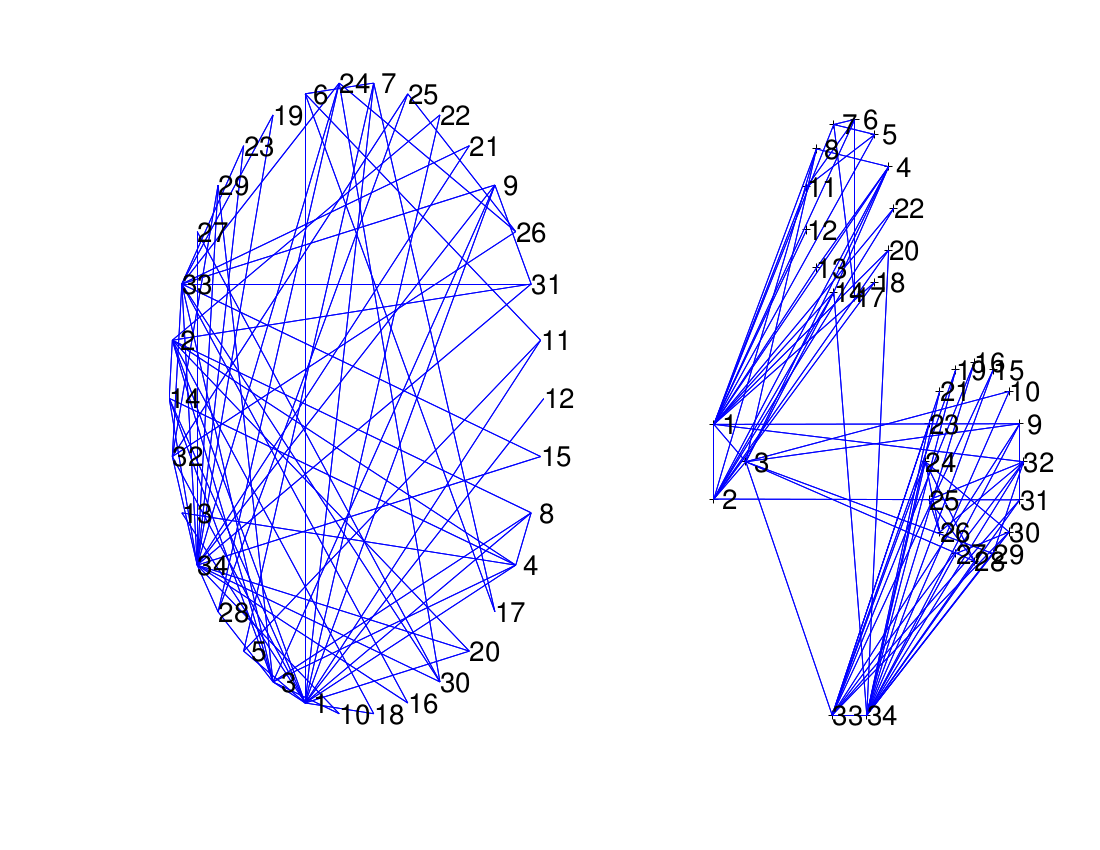
\epsfig{file = \fignet/Karate-Graph.eps, clip=, width=3.5cm,
%       height=10cm, angle=270}
%     \\
%     \\
%     \begin{tabular}{cc}
%       \begin{tabular}{p{.45\textwidth}}
%       \end{tabular}
%       &
%       \begin{tabular}{p{.5\textwidth}}
%         {\small
%           \begin{tabular}{c|rrrr}
%             (\%) & \multicolumn{4}{c}{$\widehat{\gamma}_{k\ell}$} \\
%             $k / \ell$ &  {1} & 2 & 3 &  4 \\
%             \hline
%             {1} &  {100} &   {53} &  {16} & {16} \\  
%             {2} & - &  {12} & {0} & {7}  \\  
%             3 & - & - & 8 & 73 \\
%             4 & - & - & - & 100\\
%             \hline
%             $\widehat{\pi}_{\ell}$        & 9 &  38       & 47    & 6     \\
%           \end{tabular}
%           }
%       \end{tabular}
%     \end{tabular}
%   \end{tabular}
  }


%--------------------------------------------------------------------
\subsection{Alternatives, extensions and variations}
%-------------------------------------------------------------------- 
\frame{ \frametitle{Extensions and variations}
  \paragraph{Algorithmic approaches:} Looking for communities
  \begin{itemize}
  \item Graph clustering (\refer{GiN02}, \refer{New04}); 
  \item Spectral clustering (\refer{LBB08}).
  \end{itemize}

  \bigskip\pause
  \paragraph{Variations around SBM:} 
    \begin{itemize} 
    \item Community structure (\refer{HoW08}),
    \item Mixed-membership (\refer{ABF08}), overlapping groups (\refer{LBA11a})
    \item Continuous version (\refer{DPV10}),
    \item SBM = Step-function version of $W$-random graphs (\refer{LoS06})
    \end{itemize}

  \bigskip\pause
  \paragraph{In this talk:}
  \begin{itemize}
  \item Variational inference for SBM;
  \item Variational Bayes inference for SBM;
  \item Including covariates.
  \end{itemize}
  }


%--------------------------------------------------------------------
\section{Variational inference}
\frame{\frametitle{Variational inference}}
%--------------------------------------------------------------------
\subsection{Maximum likelihood inference}
%-------------------------------------------------------------------- 
\frame{ \frametitle{Maximum likelihood inference}
  \paragraph{Maximum likelihood estimate:} We are looking for
  $$
  \widehat{\thetabf} = \arg\max_{\thetabf} \log P(\Xbf; \thetabf)
  $$
  but $P(\Xbf; \thetabf) = \sum_{\Zbf} P(\Xbf, \Zbf; \thetabf)$ is
  \emphase{not tractable}.

  \bigskip\pause
  \paragraph{Classical strategy:} Based on the decomposition
  $$
  \log P(\Xbf) = \Esp[\log P(\Xbf, \Zbf) | \Xbf] - \Esp[\log
  P(\Zbf|\Xbf) | \Xbf],
  $$
  \pause
  the EM algorithm aims at retrieving the maximum likelihood estimates via
  the alternation of 2 steps.
  \begin{description}
  \item[E-step:] calculation of $P(\Zbf|\Xbf; \widehat{\thetabf})$.
  \item[M-step:] maximisation of $\Esp[\log P(\Xbf, \Zbf; \thetabf) |
    \Xbf]$ in $\thetabf$. 
  \end{description}
  }

%-------------------------------------------------------------------- 
\frame{ \frametitle{Case of the Stochastic Block-Model}
  \paragraph{Dependency structure.}

  \bigskip
  \begin{tabular}{c|c|c}
    \begin{tabular}{p{.28\textwidth}}
      \emphase{Dependecy graph:} \\ 
      $P(\Zbf) P(\Xbf|\Zbf)$
    \end{tabular}
    &
    \begin{tabular}{p{.28\textwidth}}
      \emphase{Moral graph}  \\
      (\refer{Lau96})
    \end{tabular}
    &
    \begin{tabular}{p{.28\textwidth}}
      \emphase{Conditional dep.:} \\ 
      $P(\Zbf|\Xbf)$
    \end{tabular}
    \\
    \hline
    & & \\
    \begin{tabular}{c}
      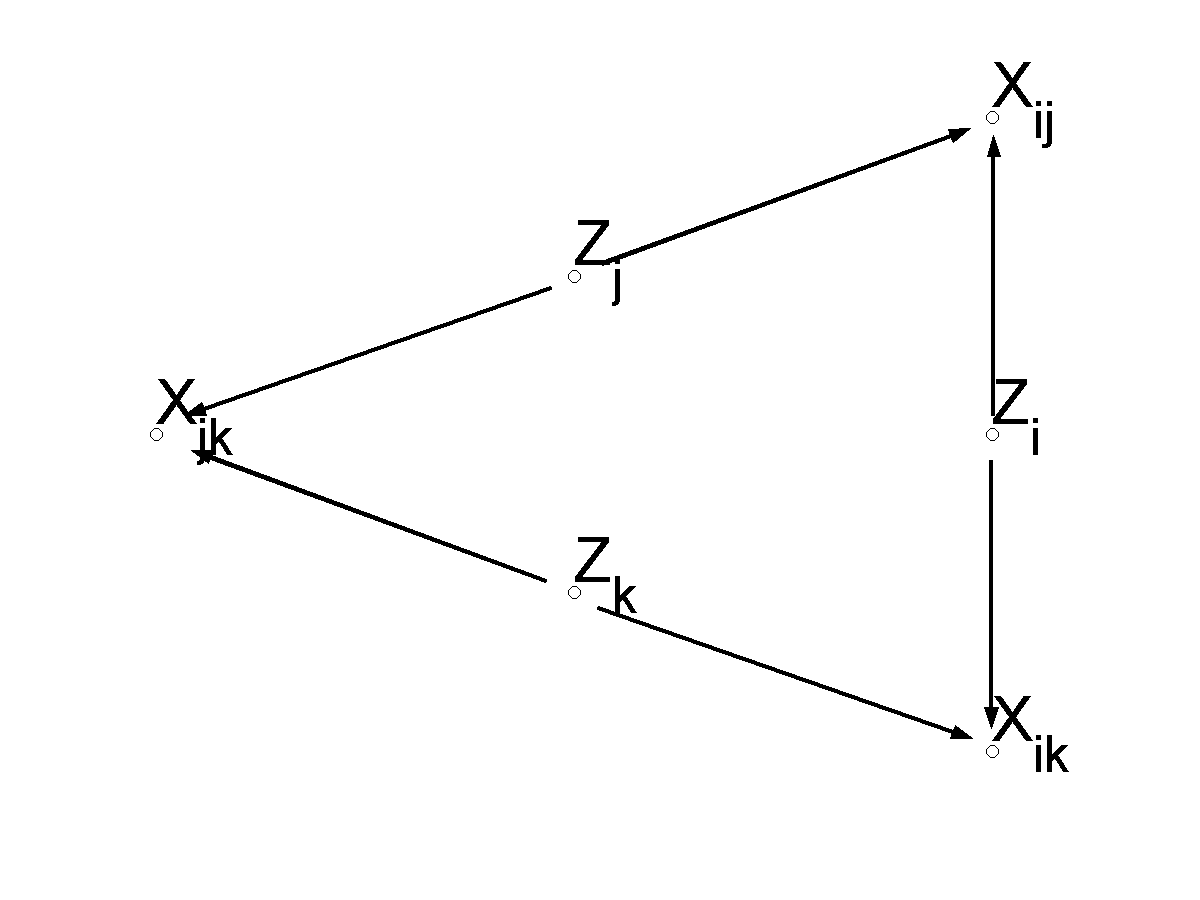
\epsfig{file=\fignet/FigNetworks-DepGraph,
      width=.25\textwidth, clip=} 
    \end{tabular}
    & 
    \begin{tabular}{c}
      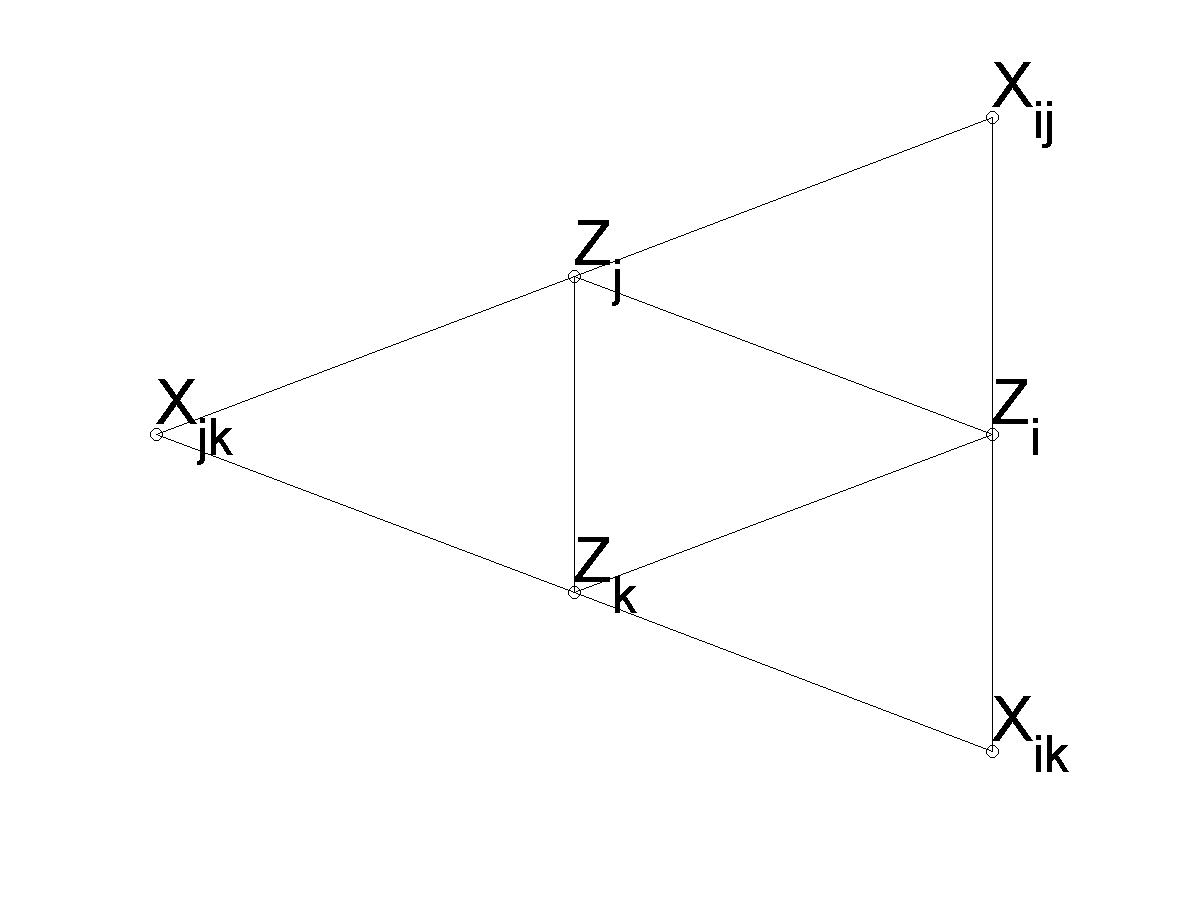
\epsfig{file=\fignet/FigNetworks-DepGraph-Moral,
      width=.25\textwidth, clip=}
    \end{tabular}
    & 
    \begin{tabular}{c}
      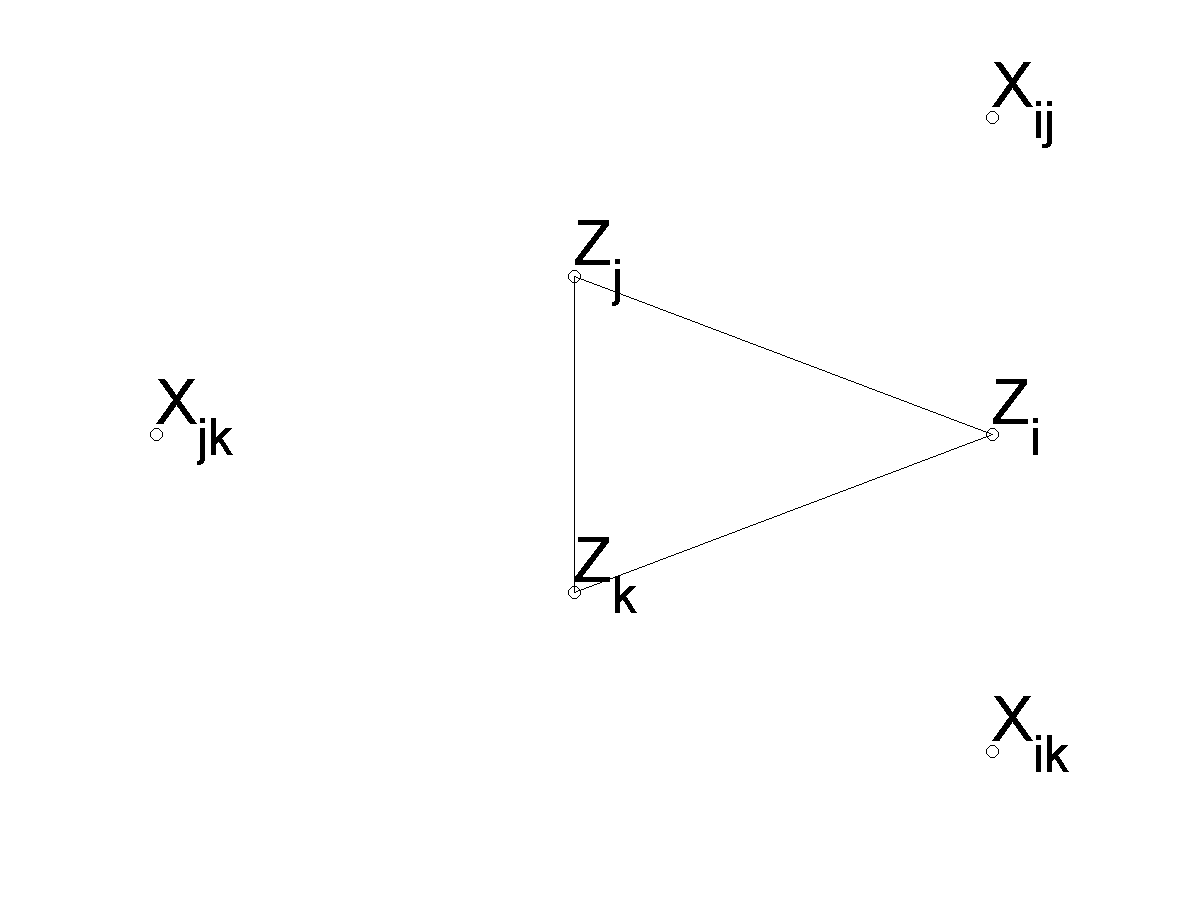
\epsfig{file=\fignet/FigNetworks-DepGraph-Conditional,
      width=.25\textwidth, clip=}
    \end{tabular} 
  \end{tabular}
  
  \bigskip\bigskip\pause
  The conditional dependency graph of $\Zbf$ is a \emphase{clique} \\
  \ra no factorisation can be hoped to calculate $P(\Zbf|\Xbf)$
  (unlike hidden Markov random fields).  
  }

%--------------------------------------------------------------------
\subsection{Variational inference}
%-------------------------------------------------------------------- 
\frame{ \frametitle{Variational approximation}

  As $P(\Zbf|\Xbf)$ can not be calculated, we need to find some
  {approximate} distribution $Q(\Zbf)$.

  \bigskip \pause
  \paragraph{Lower bound of the log-likelihood:}
  For any distribution $Q(\Zbf)$, we have (\refer{Jaa00},\refer{WaJ08}) 
  \begin{eqnarray*}
    \log P(\Xbf) & \geq & \log P(\Xbf) - \emphase{KL[Q(\Zbf); P(\Zbf|\Xbf)]} \\
    \pause \\
    & = & \Esp_Q[\log \emphase{P(\Xbf, \Zbf)}] + \Hcal(Q) 
  \end{eqnarray*}
  where $\Hcal(Q)$ is the entropy of $Q$: $\Hcal(Q) = -\Esp_Q[\log
  Q(\Zbf)]$. 

  \bigskip\bigskip\pause
  This amounts to \emphase{replace $P(\cdot|\Xbf)$ with $Q(\cdot)$} in 
  $$
  \log P(\Xbf) = \Esp_{P(\cdot|\Xbf)}[\log P(\Xbf, \Zbf)] +
  \Hcal[P(\cdot|\Xbf)]. 
  $$
  }

%-------------------------------------------------------------------- 
\frame{ \frametitle{Variational EM}
  \paragraph{'Expectation' step (pseudo E-step):}
  find the best lower bound of $\log P(\Xbf)$, i.e. the best
  approximation of $P(\cdot|\Xbf)$ as
  $$
  Q^* = \arg\min_{Q \in \Qcal} KL[Q(\Zbf); P(\Zbf|\Xbf)]
  $$
  where $\Qcal$ is a class of \emphase{'manageable' distributions}. 
% \\
%   \ra Mean-field approximation.

  \bigskip\bigskip\pause
  \paragraph{Maximisation step (M-step):} estimate $\thetabf$ as
  $$
  \widehat{\thetabf} = \arg\max_{\thetabf} \Esp_{\emphase{Q^*}}[\log P(\Xbf,
  \Zbf; \thetabf)] 
  $$
  which maximises the lower bound of $\log P(\Xbf)$.  
  }

%--------------------------------------------------------------------
\frame{ \frametitle{Approximation of $P(\Zbf|\Xbf)$ for SBM}

  We are looking for
  $$
  Q^* = \arg\min_{Q \in \Qcal} KL[Q(\Zbf); P(\Zbf|\Xbf)].
  $$

  \pause
  \begin{itemize}
%   \item The optimum over all possible distributions is
%     \emphase{$Q^*(\Zbf) = P(\Zbf|\Xbf)$} ... which can no be
%     calculated.
  \item We restrict ourselves to the set of \emphase{factorisable
      distributions}:
    $$
    \Qcal = \left\{Q: Q(\Zbf) = \prod_i Q_i(Z_i) = \prod_i \prod_k
      \tau_{ik}^{Z_{ik}}\right\}, 
    \quad
    \emphase{\tau_{ik} \approx \Pr\{Z_i=k|\Xbf\}}. \pause
    $$
  \item The optimal $\tau_{ik}^*$'s satisfy the {fix-point relation}:
  $$
  \tau_{ik}^* \propto \pi_k \prod_{j \neq i} \prod_\ell
  f_{k\ell}(X_{ij})^{\emphase{\tau^*_{j\ell}}}
  $$
  also known as \emphase{mean-field} approximation in physics
  (\refer{Par88}).
  \end{itemize}
  }

%--------------------------------------------------------------------
\subsection{Operon network}
%-------------------------------------------------------------------- 
\frame{ \frametitle{Application to a regulatory network}
  \vspace{-.5cm}\hspace{-.5cm}
  \begin{tabular}{ll}
    \begin{tabular}{p{6cm}}
      \paragraph{Regulatory network =} directed graph where
      \begin{itemize}
      \item \emphase{Nodes =} genes (or groups of genes, e.g. operons)
      \item \emphase{Edges =} regulations:
        $$
        \emphase{\{i \rightarrow j\}}
        \quad \Leftrightarrow \quad 
        \emphase{i \text{ regulates } j}
        $$
      \end{itemize}

      \onslide+<3->{
        \paragraph{Questions}
        \begin{itemize}
        \item Do some nodes share similar connexion profiles?
        \item Is there a 'macroscopic' organisation of the network?
        \end{itemize}    
        }
    \end{tabular}
    &
    \begin{tabular}{l}
      \onslide+<2->{
        \hspace{-.75cm}
        \epsfig{file=\fignet/im_EcoliVEM_NB.ps,
          width=.45\textwidth, clip=} 
        }
    \end{tabular}
  \end{tabular}
  }

%-------------------------------------------------------------------- 
\frame{ \frametitle{SBM analysis}

  \vspace{-0.5cm}
  \hspace{-0.5cm}
  \begin{tabular}{cc}      
    \begin{tabular}{p{0.45\textwidth}}
      \paragraph{Parameter estimates.} $K = 5$     \\
      \tiny{$\begin{array}{cccccc}
          \widehat{\gamma}_{k\ell}~(\%) & 1 & 2 & 3 & 4 & 5 \\
          \hline
          1 & . & . & . & . & . \\
          2 & 6.40 & 1.50 & 1.34 & . & . \\
          3 & 1.21 & . & . & . & . \\
          4 & . & . & . & . & . \\
          5 & 8.64 & 17.65 & . & 72.87 & 11.01 \\
          \hline
          \widehat{\pi}~(\%) & 65.49 & 5.18 & 7.92 & 21.10 & 0.30
        \end{array}$}
      \\ 

      \onslide+<3->{
        \paragraph{Meta-graph representation.} \\
        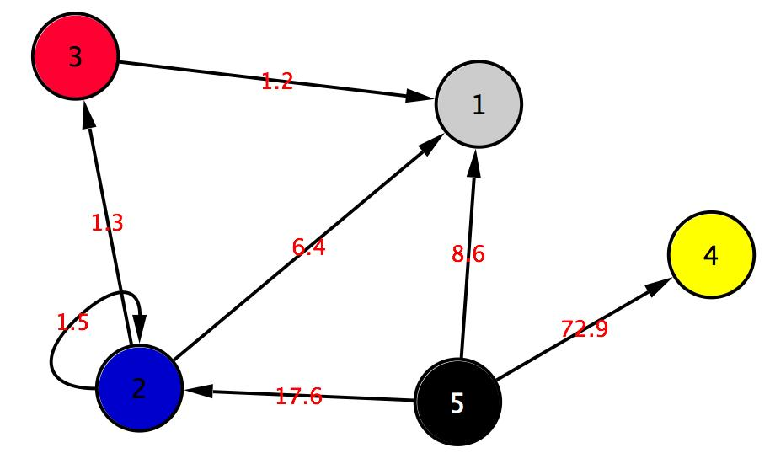
\epsfig{file=\fignet/VEMmetagraphe.ps,
          width=.4\textwidth, clip=}  \\
        }
      \\ 
      \refer{PMD09}
    \end{tabular}
    &
    \begin{tabular}{p{0.45\textwidth}}
      \onslide+<2->{
        \epsfig{file=\fignet/im_EcoliVEM_2.ps,
          width=.45\textwidth, clip=} 
        }
    \end{tabular}
  \end{tabular}
  }

%--------------------------------------------------------------------
\subsection{Consistency (?) of the variational inference}
%--------------------------------------------------------------------
\frame{ \frametitle{Properties of variational inference}

  The quality of the inference based on the variational approximation is
  not very well known yet.

  \bigskip\pause
  \paragraph{Negative result:}  (\refer{GuB05})
%   \begin{itemize}
%   \item 
  The VEM algorithm converges to a \emphase{different optimum than ML}
  in the general case, except for \emphase{'degenerated' models}.
%   \item Consistency is proved for \emphase{some incomplete data models}
%     (\refer{McT09}).
%   \item VB-EM often under-estimates the posterior variances.
%   \end{itemize}

  \bigskip\pause
  \paragraph{Specific case of graphs.}
  \begin{itemize}
  \item Specific asymptotic framework: \emphase{$n^2$ data, $'p' = n$
    'variables'} per individual.
  \item Mean field approximation is asymptotically exact for some
    models with infinite range dependency (\refer{OpW01}: law of large
    number argument).
%     $$
%     \tau_{ik}^* \propto \pi_k \prod_{j \neq i} \prod_\ell
%     f_{k\ell}(X_{ij})^{\emphase{\tau^*_{j\ell}}}
%     $$
%     $$
%     \Pr\{Z_i=k | \Xbf, \Zbf_{\emphase{\setminus i}}\} \propto \pi_k
%     \prod_{j \neq i} \prod_\ell
%     f_{k\ell}(X_{ij})^{\emphase{Z_{j\ell}}}. 
%     $$
  \end{itemize}
  }

%-------------------------------------------------------------------- 
\frame{ \frametitle{Concentration of $P(\Zbf|\Xbf)$ for binary graphs} 

  Let us denote $g$, the conditional distribution 
  $$
  g(\zbf; \Xbf) := \Pr\{\Zbf=\zbf|\Xbf\} = \frac1C \prod_i
  \pi_{Z_{i}} \prod_{j \neq i} \gamma_{Z_iZ_j}^{X_{ij}} [1 -
    \gamma_{Z_iZ_j}]^{1- X_{ij}}
  $$
%  This function is random, as it depends on $\Xbf$.

  \pause
  \paragraph{Theorem (\Refer{C�lisse,  \& al. (2011)}).} Under 
  identifiability conditions and if $\forall k, \ell: 0 < a <
  \gamma_{k\ell} < 1-a, 0 < b < \pi_k$, then we have
  $$
  \forall t>0, \qquad 
  \Pr\left\{ \left. \frac{\sum_{\zbf \neq \zbf^*} g(\zbf; \Xbf)}{g(\zbf^*;
      \Xbf)} > t \right| \Zbf = \zbf^* \right\} = \Ocal(n e^{-\kappa n}).
  $$
  \pause \ra If the true labels are $\zbf^*$, then $P(\Zbf|\Xbf)$
  concentrates around $\zbf^*$. \\
  \pause \ra SBM is a \emphase{'degenerated' model}.

  \pause \bigskip
  \paragraph{Ongoing work} about the convergence $P(\cdot|\Xbf)
  \rightarrow \delta\{\zbf^0\}$ (\Refer{Matias (2011)}).

%   \paragraph{Theorem for binary graphs:} Under conditions
%   \begin{description}
%   \item[C1:] $\forall k \ne k', \quad \exists \ell: \quad
%     \gamma_{k\ell} \ne \gamma_{k'\ell} \quad \text{or} \quad
%     \gamma_{\ell k} \ne \gamma_{\ell k'}$;
%   \item[C2:] $\exists a>0: \quad
%     \min_{k, \ell}(\gamma_{k\ell},1-\gamma_{k\ell})>a$;
%   \item[C3:] $\exists b>0: \quad \min_k  \pi_{k} >b$;
%   \end{description}
%   when $n \rightarrow \infty$
%   $$ 
%   \forall t>0,  \;  \Pr_{\Xbf|\Zbf=\zbf^*} \left\{ \frac{ \Pr\{\Zbf \ne
%       \zbf^* | \Xbf\} }{ \Pr\{\Zbf=\zbf^*| \Xbf\}} >t \right\}
%   \rightarrow 0
%   $$  \pause

%   \bigskip
%   \paragraph{Corollary:}
%   $$
%   \mathcal{L}(P_{\Xbf|\Zbf=\zbf^*}(\Zbf | \Xbf))
%   \underset{n \rightarrow \infty}{\longrightarrow} \delta (\zbf^*).
%   $$
  }

% %-------------------------------------------------------------------- 
% \frame{ \frametitle{Sketch of proof}
%   \begin{itemize}
%   \item $\Pr\{\Zbf=\zbf | \Xbf\}=P(\Xbf|\Zbf=\zbf)\Pr\{\Zbf=\zbf\} /
%     P(\Xbf)$ depends on $\Xbf$; \pause
%   \item The ratio $\Pr\{\Zbf \ne \zbf^* | \Xbf\} / \Pr\{\Zbf=\zbf^*|
%     \Xbf\}$ \emphase{eliminates $P(\Xbf)$}; \pause
%   \item We have
%     $$
%     P(\Xbf| \Zbf=\zbf)\Pr\{\Zbf=\zbf\}=\prod_{i\neq j}
%     \gamma_{z_iz_j}^{x_{ij}}(1-\gamma_{z_iz_j})^{(1-x_{ij})}\prod_{i}
%     \pi_{z_i}
%     $$
%     so $\emphase{\log} \left[\Pr\{\Zbf = \zbf | \Xbf\} / \Pr\{\Zbf=\zbf^*|
%       \Xbf\}\right]$ is a \emphase{sum of $n^2$ terms}; \pause
%   \item Bernstein inequality implies that the concentration rate
%     of the above function to its mean is of \emphase{order $n^2$}; \pause
%   \item $\Pr\{\Zbf \ne \zbf^* | \Xbf\}=\sum_{\zbf \neq \zbf^*} \Pr\{\Zbf
%     =\zbf | \Xbf\}$ is a \emphase{sum of $K^n=e^{n\log K}$ terms}; \pause
%   \item $n^2$ wins against $n$.
%   \end{itemize}
%   \Refer{Celisse, Daudin, Pierre, 11}
%   }

%-------------------------------------------------------------------- 
\frame{ \frametitle{Concentration of the degree distribution} 

  \vspace{-1cm}
  \begin{tabular}{cc}
    \begin{tabular}{p{0.5\textwidth}}
      \bigskip
      \paragraph{Binary graph.} 
      Binomial distribution of the degrees
      $$
      K_i|(i \in q) \sim \Bcal(n-1, \overline{\gamma}_k)
      $$
      where $\overline{\gamma}_k = \sum_{\ell} \pi_\ell \gamma_{k,
        \ell}$. 

      \bigskip \onslide+<2->{
        \paragraph{Normalised degree:} 
        $
        D_i = K_i / (n-1)
        $
        concentrates around $\overline{\gamma}_k$.
        }

      \bigskip \onslide+<6->{
        \paragraph{Linear algorithm} 
        \begin{itemize}
        \item based on the gaps between the ordered $D_{(i)}$,
        \item provides consistent estimates of $\pibf$ and $\gammabf$
          can be derived.
        \end{itemize}
        (\Refer{Channarond (2011)}).
        }
    \end{tabular}
    &
    \hspace{-0.5cm} 
    \onslide+<3->{
      \begin{tabular}{p{0.5\textwidth}}
        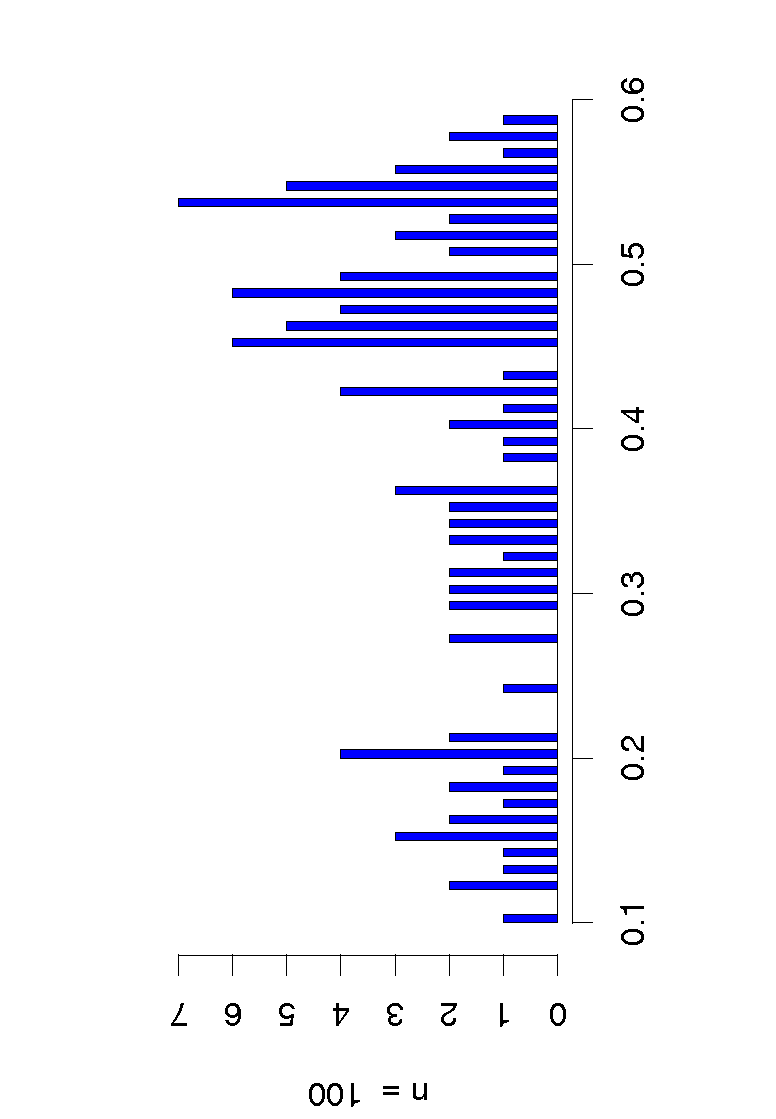
\epsfig{file=\fignet/ConcentrBinom-n100, angle=270,
          width=.45\textwidth, clip=} \\ 
        \vspace{-1.5cm}
        }
      \onslide+<4->{
        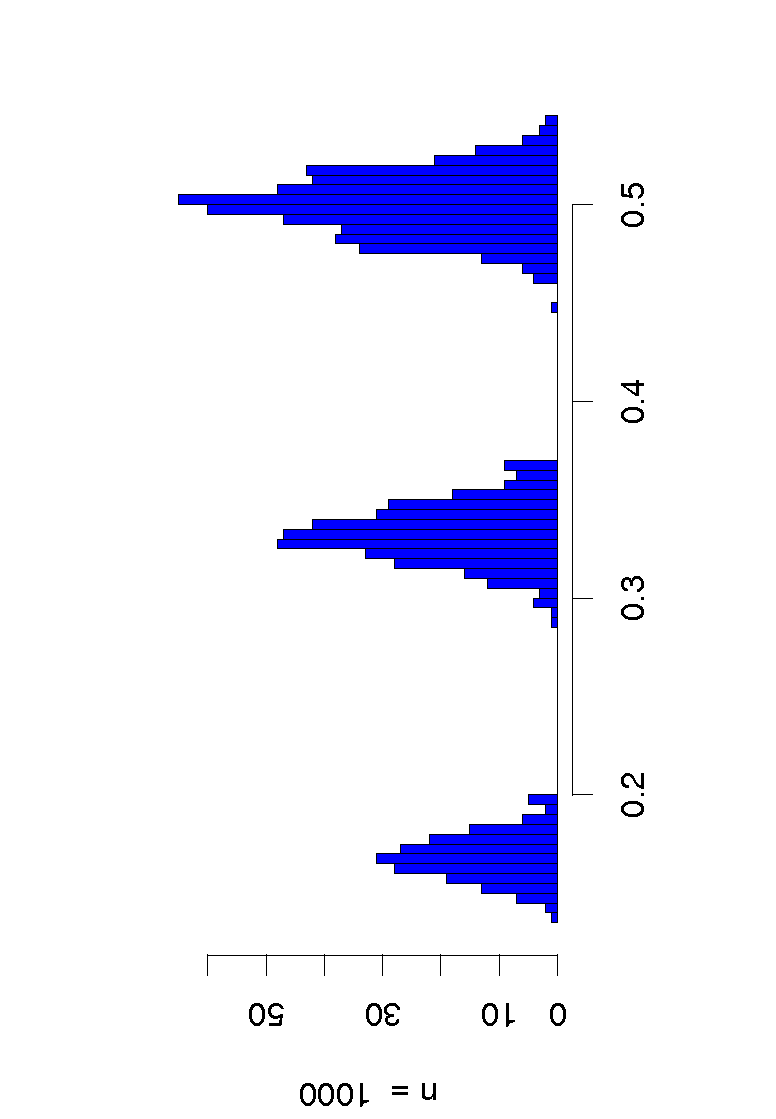
\epsfig{file=\fignet/ConcentrBinom-n1000, angle=270,
          width=.45\textwidth, clip=} \\ 
        \vspace{-1.5cm}
        }
      \onslide+<5->{
        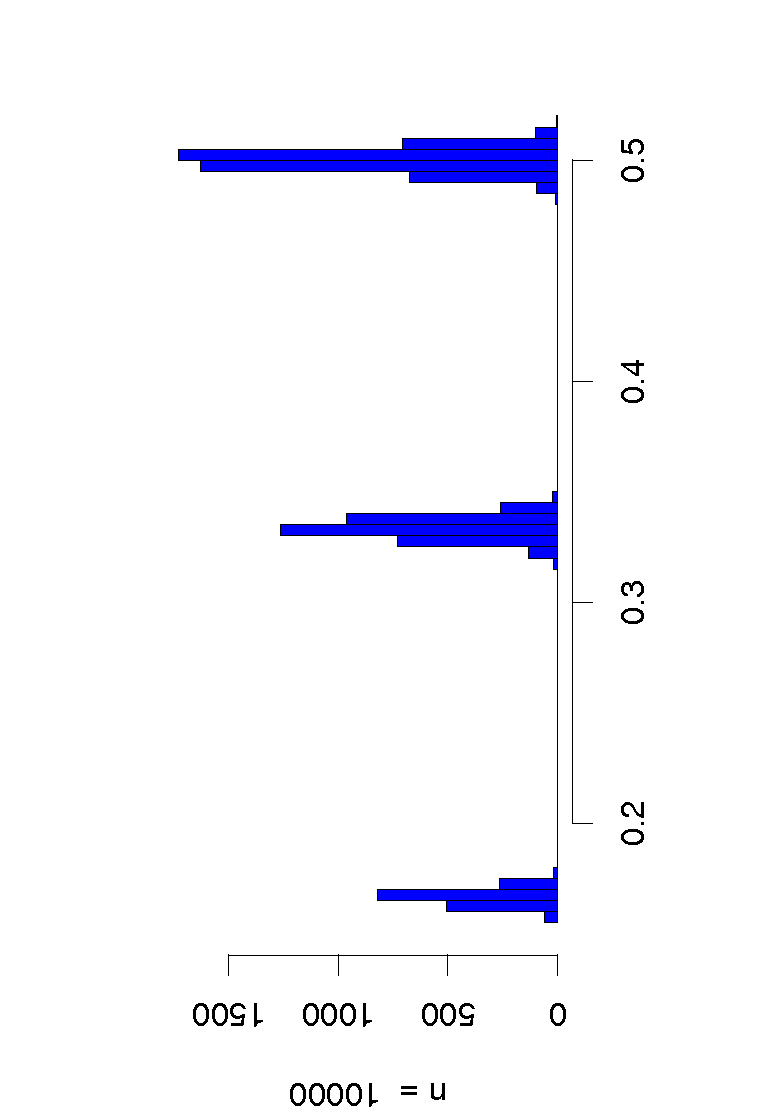
\epsfig{file=\fignet/ConcentrBinom-n10000, angle=270,
          width=.45\textwidth, clip=} 
        }
    \end{tabular}
  \end{tabular}     
  }
  
%--------------------------------------------------------------------
\section{Variational Bayes inference}
\frame{ \frametitle{Variational Bayes inference}}
%--------------------------------------------------------------------
\subsection{Variational Bayes approximation}
%-------------------------------------------------------------------- 
\frame{ \frametitle{Variational Bayes inference} 

  \paragraph{Bayesian setting:} Both $\thetabf$ and $\Zbf$ are
  random and unobserved and we want to retrieve \emphase{$P(\Zbf,
    \thetabf|\Xbf)$} 
  \pause 
  so we look for 
  $$
  Q^* = \arg\min_{Q \in \Qcal} KL[Q(\Zbf, \thetabf); P(\Zbf,
  \thetabf|\Xbf)]
  $$
  within $\Qcal = \{Q: Q(\Zbf, \thetabf) =
  \emphase{Q_Z}(\Zbf)\emphase{Q_\theta}(\thetabf)\}$. 

  \bigskip\pause
  \paragraph{VB-EM algorithm:} In the exponential family / conjugate
  prior context
  $$
  P(\Xbf, \Zbf, \thetabf) \propto \exp\{\phi(\thetabf)' [u(\Xbf,
  \Zbf) + \nubf]\} \pause
  $$
  the optimal $Q^*(\Zbf, \thetabf)$ is recovered (\refer{BeG03}) via
  \begin{eqnarray*}
    \emphase{\text{pseudo-M:} \quad Q_{\thetabf}}(\thetabf) 
    & \propto 
    & \exp \left(\phi(\thetabf)'
      \left\{\Esp_{\emphase{Q_Z}}[u(\Xbf, \Zbf)] + \nubf \right\}
      \right) \\ 
    \emphase{\text{pseudo-E:} \quad Q_Z}(\Zbf)     
    & \propto     
    & \exp \{ \Esp_{\emphase{Q_\theta}}[\phi(\thetabf)]' u(\Xbf, \Zbf) \}   
    \pause
  \end{eqnarray*}
  See \refer{LBA10} for binary SBM inference.
  }

%--------------------------------------------------------------------
\subsection{Operon network}
%-------------------------------------------------------------------- 
\frame{ \frametitle{Operon network: Comparison of {\VEM} and {\VBEM}}
%   Network are n = 338 operons, linked if one encodes a
%   transcription factor that directly regulates the other one. 
  {\VEM} estimates for the $K=5$ group model lie within the {\VBEM}
  approximate 90\% credibility intervals (\refer{GDR11}). 

  {\footnotesize
    $$
    \begin{tabular}{cccccc}
      $\gamma_{k\ell}$ & 1 & 2 & 3 & 4 & 5 \\
      \hline 
      1 & 0.03 & 0.00 & 0.03 & 0.00 & 0.00 \\
      2 & 6.40 & 1.50 & 1.34 & 0.44 & 0.00 \\
      3 & 1.21 & 0.89 & 0.58 & 0.00 & 0.00 \\
      4 & 0.00 & 0.09 & 0.00 & 0.95 & 0.00 \\
      5 & 8.64 & 17.65 & 0.05 & 72.87 & 11.01 \\
      \hline
      $\pi$ & 65.49 & 5.18 & 7.92 & 21.10 & 0.30 \\
      \hline \hline 
      \onslide+<2->{ 
        1 & [0.02;0.04] & [0.00;0.10] & [0.01;0.08] & [0.00;0.03] &
      [0.02;1.34] \\  
        2 & [6.14;7.60] & [0.61;3.68] & [1.07;3.50] & [0.05;0.54] &
      [0.33;17.62] \\  
        3 & [1.20;1.72] & [0.35;2.02] & [0.56;1.92] & [0.03;0.30] &
      [0.19;10.57] \\  
        4 & [0.01;0.07] & [0.04;0.51] & [0.01;0.20] & [0.76;1.27] &
      [0.08;4.43] \\  
        5 & [6.35;12.70] & [4.60;33.36] & [4.28;24.37] & [63.56;81.28]
      & [5.00;95.00] \\  
        \hline 
        $\pi$ & [59.65;74.38]&  [2.88;6.74] & [5.68;10.77] &
      [16.02;24.04] & [0.11;1.42] 
      }
      \end{tabular} 
    $$
    }
  
  \onslide+<2->{
    {\VEM} and {\VBEM} estimates for the $K=5$ group model (approximate
    90\% credibility intervals).
    }
  }

%--------------------------------------------------------------------
\frame{ \frametitle{Approximate posterior distribution $Q^*_\theta$}

  \vspace{-0.5cm}
  $$
  \begin{tabular}{c}
    \includegraphics[width=.7\textwidth]{../Figures/im-pi1BVEM}\\        
    \includegraphics[width=.7\textwidth]{../Figures/im-pi2BVEM}\\
    \includegraphics[width=.7\textwidth]{../Figures/im-pi3BVEM}\\
    \includegraphics[width=.7\textwidth]{../Figures/im-pi4BVEM}\\
    \includegraphics[width=.7\textwidth]{../Figures/im-pi5BVEM}\\
    \hline 
    \includegraphics[width=.7\textwidth]{../Figures/im-alphaBVEM}\\
  \end{tabular}
  $$
  }

%--------------------------------------------------------------------
\subsection{Quality of the variational Bayes approximation}
%-------------------------------------------------------------------- 
\frame{ \frametitle{Variational Bayes approximation: Simulation Study}

  Few is known about the properties of variational-bayes inference:
  \begin{itemize}
  \item Consistency is proved for \emphase{some incomplete data models}
    (\refer{McT09}).
  \item In practice, VB-EM often under-estimates the posterior variances.
  \end{itemize}

  \bigskip\pause
  \paragraph{Simulation design:} 
  \begin{itemize}
  \item \pause 2-group binary SBM with parameters with 2 scenarios
    $$
    \pi=\left(\begin{array}{cc}
        0.6 & 0.4
      \end{array}\right),  
    \qquad
    \gamma=\left(\begin{array}{cc}
        0.8 & 0.2 \\
        0.2 & \emphase{0.5/0.3}
      \end{array}\right)
    $$
  \item \pause Comparison of 4 methods: EM (when possible), {\VEM}, BP and
    {\VBEM}
%     ($n = 18$: because of the computation time required by for EM). 
  \item \pause Belief Propagation (BP) algorithm: 
%     Provides a specific approximation for the second term in
    $$
    \Esp_Q[\log P(\Xbf, \Zbf)] = \sum_{i, k}
    \underset{\emphase{\normalsize
        \tau_{ik}}}{\underbrace{\Esp_Q[Z_{ik}]}} \log \pi_k + \sum_{i,
      j} \sum_{k, \ell} \underset{\emphase{\normalsize
        \Delta_{ijk\ell} \neq
        \tau_{ik}\tau_{j\ell}}}{\underbrace{\Esp_Q[Z_{ik} Z_{j\ell}]}}
    \log f(X_{ij}; \gamma_{k\ell}).
    $$
  \item \pause 500 graphs are simulated for each scenario and each graph
    size.
  \end{itemize}
  }

%--------------------------------------------------------------------
\frame{ \frametitle{Estimates, standard deviation and likelihood}

  \paragraph{Comparison on small graphs ($n = 18$):}
  {\small
    \begin{tabular}{ccccccccc} 
      & $\pi_1$ & $\gamma_{11}$ & $\gamma_{12}$ & $\gamma_{22}$ &
      $\log P(X)$ \\   
      \hline
      \emphase{Scenario 1} & 60\% & 80\% & 20\% & 50\% & \\ 
      \hline 
      EM & 59.1 (13.1) & 78.5 (13.5) & 20.9 (8.4) & 50.9 (15.4) & -90.68 \\  
      {\VEM} & 57.7 (16.6) & 78.8 (12.4) & 22.4 (10.7) & 50.3 (14.6) & -90.87\\  
      BP & 57.9 (16.2) & 78.9 (12.3) & 22.2 (10.5) & 50.3 (14.5) & -90.85 \\  
      {\VBEM} & 58.1 (13.3) & 78.2 (9.7) & 21.6 (7.7) & 50.8 (13.3) & -90.71 \\ 
      \hline \\
      \hline
      \emphase{Scenario 2} & 60\% & 80\% & 20\% & 30\% &  \\ 
      \hline
      EM & 59.5 (14.1) & 78.7 (15.6) & 21.2 (8.7) & 30.3 (14.3) & -88.18 \\  
      {\VEM} & 55.6 (19.0) & 80.1 (14.0) & 24.0 (11.8) & 30.8 (13.8) & -88.54 \\  
      BP & 56.6 (17.8) & 80.0 (13.6) & 23.2 (11.0) & 30.8 (13.8) & -88.40 \\  
      {\VBEM} & 58.4 (14.6) & 77.9 (12.0) & 22.3 (9.3) & 32.1 (12.3) & -88.26 \\  
    \end{tabular} 
    }
  \bigskip\pause
  \begin{itemize}
  \item All methods provide similar results.
  \item {\EM} achieves the best ones.
  \item Belief propagation ({\BP}) does not significantly improve {\VEM}.
  \end{itemize}
  }

%--------------------------------------------------------------------
\frame{ \frametitle{Influence of the graph size}
  Comparison of \textcolor{red}{{\VEM}: $\bullet$} and
  \textcolor{blue}{{\VBEM}: $+$} in scenario 2 (most difficult). \\
  Left to right: $\pi_1$, $\gamma_{11}$, $\gamma_{12}$, $\gamma_{22}$.

  \bigskip
  \emphase{Means.} \\
  \includegraphics[width=1\textwidth]{../Figures/im-etudnVB1} \\
  
  \pause
  \emphase{Standard deviations.} \\
  \includegraphics[width=1\textwidth]{../Figures/im-etudnVB2}
  
  \begin{itemize}
  \item {\VBEM} estimates converge more rapidly than {\VEM} estimates.
  \item Their precision is also better.
  \end{itemize}
  }

%--------------------------------------------------------------------
\frame{ \frametitle{{\VBEM} Credibility intervals}

  \paragraph{Actual level as a function of $n$:}   $\pi_1$: $+$,
  $\gamma_{11}$: \textcolor{red}{$\triangle$}, $\gamma_{12}$:
  \textcolor{blue}{$\circ$}, $\gamma_{22}$: \textcolor{green}{$\bullet$}
  $$
  \includegraphics[width=1\textwidth]{../Figures/im-ICQ2-2-new} 
  $$

  \pause
  \begin{itemize}
  \item For all parameters, {\VBEM} posterior credibility intervals
    achieve the nominal level (90\%), as soon as $n \geq 30$.
  \item \ra \emphase{The {\VBEM} approximation seems to work well}.
%   \item These may be due to the concentration of $P(Z|X)$ around the
%     true value of $Z$ (work in progress).
  \end{itemize}
  }

%--------------------------------------------------------------------
\frame{ \frametitle{Convergence rate of the {\VBEM} estimates}
  \emphase{Width of the posterior credibility intervals.}
  {$\pi_1$}, \textcolor{red}{$\gamma_{11}$},
  \textcolor{blue}{$\gamma_{12}$}, \textcolor{green}{$\gamma_{22}$}
  \\
  \includegraphics[width=1\textwidth]{../Figures/im-ICQ2-3} \\

  \pause
  \begin{itemize}
  \item The width decreases as $1/\sqrt{n}$ for $\pi_1$.
  \item It decreases as $1/n = 1/sqrt{n^2}$ for $\gamma_{11}$,
    $\gamma_{12}$ and $\gamma_{22}$.
  \item Consistent with the penalty of the ICL criterion
    proposed by \refer{DPR08} (see next slide).
  \end{itemize}
  }

% %--------------------------------------------------------------------
% \frame{ \frametitle{Why does {\VBEM} work so well? (off the record)}
% %-------------------------------------------------------------------- 
%   \emphase{Work in progress:} Daudin \& Celisse are about to prove the 
%   concentration of $P(Z|X)$ around the true value $z^*$, i.e.
%   $$
%   P(Z|X) \underset{n \rightarrow \infty}{\longrightarrow} \delta_{z^*}(Z)
%   $$
%   \bigskip
%   \emphase{Intuition:} If this holds, 
%   \begin{enumerate}[($i$)]
%   \item The limit distribution $\delta_{z^*}(Z)$ belongs to the
%     distribution class over which {\VBEM} approximation achieves
%     maximisation, so it is reached;
%   \item The joint conditional distribution $P(\theta, Z|X) =
%     P(\theta|Z, X) P(Z|X)$ tends to $P(\theta|Z, X) \delta_{z^*}(Z)$.
%     Again $P(\theta|Z, X)$ belongs to the distribution class of
%     {\VBEM}, so it is also reached;
%   \end{enumerate}
%   And the variational approximation tends to be ... exact.
%   }


%-------------------------------------------------------------------- 
\frame{ \frametitle{Few more about inference} 
  \paragraph{Identifiability.} Even for binary edges, MixNet (SBM) is
  identifiable (\refer{AMR09}) ... although mixtures of Bernoulli are
  not.

  \bigskip\bigskip\pause
  \paragraph{Model selection.} 
  \begin{itemize}
  \item \refer{DPR08} propose the penalised criterion
    $$
    ICL(K) = \Esp_{Q^*}[\log P(\Zbf, \Xbf)] - \frac12 \left\{(K-1)\log n + K^2
      \log[n(n-1)/2]\right\}.
    $$
  \item \pause The difference between ICL and BIC is the \emphase{entropy
      term $\Hcal(Q^*)$} ... which is almost zero (due to the
    concentration of $P(\Zbf|\Xbf)$).
  \item \pause BIC and ICL-like criteria are also considered in
    \refer{LBA11b} for SBM in the context of variational Bayes
    inference.
  \end{itemize}

%   \bigskip\bigskip\pause
%   \paragraph{Model averaging.} For a parameter $\delta$ not directly
%   depending on $K$, BMA suggests to consider 
%   $$
%   \widetilde{\delta} = \sum_K \emphase{P(K|\Xbf)}
%   \widehat{\delta}^K.
%   $$
%   \ra Optimal approximation of $P(K|\Xbf)$ can be derived in the
%   variational Bayes context (\Refer{Volant \& al}).
 }
  
%--------------------------------------------------------------------
\section{Covariates in valued networks}
\frame{ \frametitle{Covariates in valued networks}}
%--------------------------------------------------------------------
\subsection{Accouting for covariates}
%--------------------------------------------------------------------

\frame{ \frametitle{Valued network}
  \paragraph{Understanding the mixture components:} Observed clusters
  may be related to exogenous covariates. 
%   \ra Including such covariates enlightens \emphase{residual
%     heterogeneity}.

  \bigskip
  \paragraph{Model-based clustering}  (such as SBM) provide a
  comfortable set-up to account for covariates.

  \bigskip\bigskip\pause
  \paragraph{Generalised linear model.} In the context of exponential
  family, covariates $\ybf$ can be accounted for via a regression term
  $$
  g(\Esp X_{ij}) = \mu_{k\ell} + \ybf_{ij} \emphase{\betabf}, 
  \qquad \text{if } Z_{ik} Z_{j\ell} = 1
  $$
  where \emphase{$\betabf$ does not depend on the group}
  (\refer{MRV10}).
  
  \bigskip\bigskip\pause 
  Both VEM or VBEM inference can be performed.
%  (with only a \emphase{(slight) modification of the M-step}).  
  }

%--------------------------------------------------------------------
\frame{ \frametitle{Tree interaction network}
  \begin{tabular}{cc}
    \hspace{-.5cm}
    \begin{tabular}{p{.4\textwidth}}
      \paragraph{Data:} $n = 51$ tree species, \\
      $X_{ij}=$ number of shared parasites (\refer{VPD08}).

      \onslide+<2->{
        \bigskip
        \paragraph{Model:}
        $$
        X_{ij} \sim \Pcal(\lambda_{k\ell}),
        $$
        $\lambda_{k\ell} =$ mean number of shared parasites.
        
        \bigskip
        \paragraph{Results:} ICL selects $K=7$ groups}
      \onslide+<3->{
        that are \emphase{strongly related with phylums}. 
        }
      \end{tabular}
    & 
    \hspace{-.75cm}
    \begin{tabular}{c}
      \onslide+<2->{
        {\tiny
          \begin{tabular}{c|ccccccc}
            $\widehat{\lambda}_{k\ell}$ & T1 & T2 & T3 & T4 & T5 & T6 &
            T7 \\ 
            \hline
            T1 & 14.46 & 4.19 & 5.99 & 7.67 & 2.44 & 0.13 & 1.43 \\
            T2 &  & 14.13 & 0.68 & 2.79 & 4.84 & 0.53 & 1.54 \\
            T3 &  &  & 3.19 & 4.10 & 0.66 & 0.02 & 0.69 \\
            T4 &  &  &  & 7.42 & 2.57 & 0.04 & 1.05 \\
            T5 &  &  &  &  & 3.64 & 0.23 & 0.83 \\
            T6 &  &  &  &  &  & 0.04 & 0.06 \\
            T7 &  &  &  &  &  &  & 0.27 \\
            \hline \hline
            $\widehat{\pi}_k$ & 7.8 & 7.8 & 13.7 & 13.7 & 15.7 & 19.6 &
            21.6  
          \end{tabular}
          }\\
        }
      \onslide+<3->{
        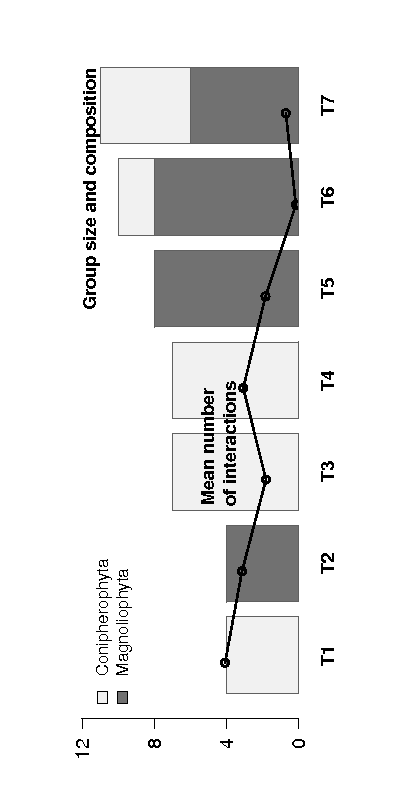
\epsfig{file=\fignet/MRV10_AoAS_Q7_group.eps, width=.5\textheight,
          height=.5\textwidth, clip=, angle=270}
        }
    \end{tabular}
  \end{tabular}
  }

%--------------------------------------------------------------------
\frame{ \frametitle{Accounting for taxonomic distance}
  \begin{tabular}{cc}
    \hspace{-.5cm}
    \begin{tabular}{p{.4\textwidth}}
      \paragraph{Model:}
      $$
      X_{ij} \sim \Pcal(\lambda_{k\ell} \emphase{e^{\beta d_{ij}}}).
      $$

      \bigskip\pause
      \paragraph{Results:} $\widehat{\beta} = -0.317$. \\
      \ra for $\overline{d} = 3.82$, 
      $$
      e^{\widehat{\beta}\overline{d}} = .298
      $$
      \ra The mean number of shared parasites \emphase{decreases with
        taxonomic distance}.
      \pause
    \end{tabular}
    & 
    \hspace{-.75cm}
    \begin{tabular}{c}
      {\tiny
        \begin{tabular}{c|cccc}
          $\widehat{\lambda}_{k\ell}$ & T'1 & T'2 & T'3 & T'4 \\ 
          \hline
          T'1 & 0.75 & 2.46 & 0.40 & 3.77 \\
          T'2 &  & 4.30 & 0.52 & 8.77 \\ 
          T'3 &  &  & 0.080 & 1.05 \\ 
          T'4 &  &  &  & 14.22 \\
          \hline \hline
          $\widehat{\pi}_k$ & 17.7 & 21.5 & 23.5 & 37.3 \\
          \hline \hline
          $\widehat{\beta}$ & \multicolumn{4}{c}{-0.317}
        \end{tabular}
        } \\ 
      \pause
      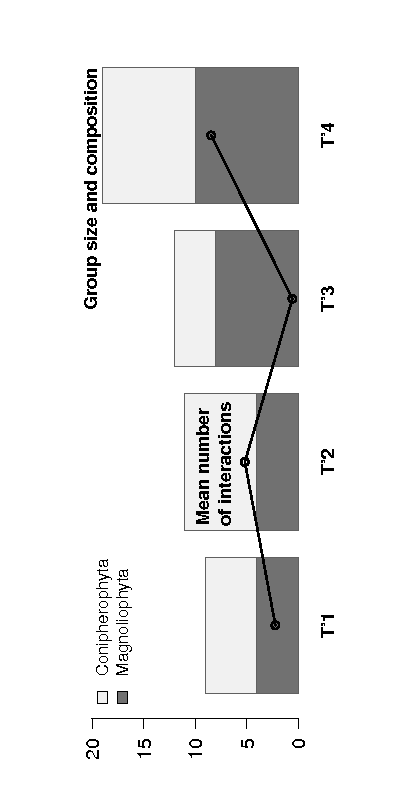
\epsfig{file=\fignet/MRV10_AoAS_Q4_group.eps, width=.5\textheight,
        height=.5\textwidth, clip=, angle=270}
    \end{tabular}
  \end{tabular}
  
  \ra Groups are no longer associated with the phylogenetic
  structure. \\
  \ra Mixture $=$ \emphase{residual heterogeneity} of the regression.
  }

%--------------------------------------------------------------------
\frame{ \frametitle{Comparison of classifications and G-O-F}
  \begin{tabular}{cc}
    \hspace{-.5cm}
    \begin{tabular}{p{.5\textwidth}}
      Accounting for taxonomy deeply modifies the group structure: 
      {\footnotesize
        $$
        \begin{tabular}{c|cccc}
          & T'1 & T'2 & T'3 & T'4 \\
          \hline
          T1 & - & -   &  -  &  4  \\
          T2 & - & -   &  -  &  4  \\
          T3 & 2 & 5   &  -  &  -  \\
          T4 & - & 2   &  -  &  5  \\
          T5 & - & 2   &  -  &  6  \\
          T6 & - & -   & 10  &  -  \\
          T7 & 7 & 2   &  2  &  -
        \end{tabular} 
        $$
        }\pause

      \bigskip
      \paragraph{Goodness of fit} can be assessed via the predicted intensities
      $\widehat{X}_{ij}$ or degrees $\widehat{K}_{i}$.
    \end{tabular}
    & 
    \hspace{-.5cm}
    \begin{tabular}{p{.5\textwidth}}
      \paragraph{Edges $X_{ij}$:} \\
      \epsfig{file=\fignet/MRV10_AoAS_FitX_Q4.eps, width=.35\textwidth,
        clip=}

      \paragraph{Degrees $K_i$:} \\
      \epsfig{file=\fignet/MRV10_AoAS_FitK_Q4.eps, width=.35\textwidth,,
        clip=}
    \end{tabular}
  \end{tabular}
  }

%--------------------------------------------------------------------
\section{Conclusion}
\frame{ \frametitle{Conclusion}}
%--------------------------------------------------------------------
\subsection{Conclusion}
%--------------------------------------------------------------------
\frame{ \frametitle{Conclusion}

  \paragraph{Stochastic block-model:} flexible and already widely used
  mixture model to uncover some underlying heterogeneity in networks.

  \bigskip\pause
  \paragraph{Variational inference}
  \begin{itemize}
  \item \emphase{Efficient and scalable} (\Refer{Daudin (2011)}: $n >
    2000$) in terms of computation times (as opposed to MCMC).
  \item Seems to work well, because the conditional distribution
    $P(\Zbf|\Xbf)$ (and therefore $P(\Zbf, \thetabf|\Xbf)$)
    \emphase{asymptotically belongs to the class $\Qcal$} within which
    the optimisation if achieved.
  \item Due to the \emphase{specific asymptotic framework} of
      networks.
  \end{itemize}

  \bigskip\pause
  \paragraph{Alternative methods.} Faster algorithms do exist for
  large graphs:
  \begin{itemize}
  \item Based on the degree distribution (\Refer{Channarond (2011))}
  \item Based on spectral clustering (\refer{RCY10}).
  \end{itemize}
  }

%--------------------------------------------------------------------
\subsection{Future work}
%--------------------------------------------------------------------
\frame{ \frametitle{Future work}

  \paragraph{Theoretical properties of variational estimates.}
  Although the graph context seems favourable, we still need more
  understanding about variational and variational Bayes inference
  properties. 

  \bigskip\pause
  \paragraph{SBM = discrete version of $W$-graph.} Let 
  \begin{eqnarray*}
    \phi :  [0 ,1]^2 & \rightarrow & [0, 1] \\
    \{Z_i\} \text{ i.i.d.} & \sim & \Ucal[0, 1] \\
    \{X_{ij}\} \text{ indep.} | \{Z_i\} & \sim & \Bcal[\phi(Z_i,
    Z_j)]
  \end{eqnarray*}
  \begin{itemize}
  \item Approximation of the $\phi(u, v)$ function by a step function
    $\gamma_{k\ell}$ (SBM)
  \item Model averaging based on optimal variational weights
    (\Refer{Volant (2011)})
  \end{itemize}
  }

%--------------------------------------------------------------------
\subsection{Acknowledgements}
%--------------------------------------------------------------------
\frame{ \frametitle{Acknowledgements}

  \paragraph{People:} \\
  A.~C�lisse, A.~Channarond, J.-J.~Daudin, S.~Gazall, M.~Mariadassou,
  V.~Miele, F.~Picard, C.~Vacher



  \bigskip
  \paragraph{Grant:} \\
  Supported by the French Agence Nationale de la
  Recherche \\
  \centerline{\emphase{NeMo} project ANR-08-BLAN-0304-01}  
  \pause

  \bigskip
  \paragraph{Softwares:}
  \begin{itemize}
  \item Stand-alone \emphase{MixNet}: \\
    \centerline{\url{stat.genopole.cnrs.fr/software/mixnet/}}
  \item R-package \emphase{Mixer}: \\
    \centerline{\url{cran.r-project.org/web/packages/mixer/index.html}}
  \item R-package \emphase{NeMo}: Network motif detection \\
    in preparation
  \end{itemize}
  }


%--------------------------------------------------------------------
{\tiny
  \bibliography{/Biblio/ARC} %,/Biblio/AST,/Biblio/SSB}
  \bibliographystyle{/Latex/astats}
  %\bibliographystyle{plaine}
  }

%--------------------------------------------------------------------
%--------------------------------------------------------------------
\end{document}
%--------------------------------------------------------------------
%--------------------------------------------------------------------

  \begin{tabular}{cc}
    \hspace{-.5cm}
    \begin{tabular}{p{.5\textwidth}}
    \end{tabular}
    & 
    \hspace{-.5cm}
    \begin{tabular}{p{.5\textwidth}}
    \end{tabular}
  \end{tabular}


\message{ !name(NeuriImag-1111-SBM.tex) !offset(-1346) }
